%%%%%%%%%%%%%%%%%%%%%%%%%%%%%%%%%%%%%%%%%%%%%%%%%%%%%%%%%%%%%%%%%%%%%
\section{Process Description}
We now apply the path-following NMPC to a more relevant example: an isothermal reactor and separator process shown in Figure \ref{fig:process}.
	\begin{figure}[H]
		\centering
		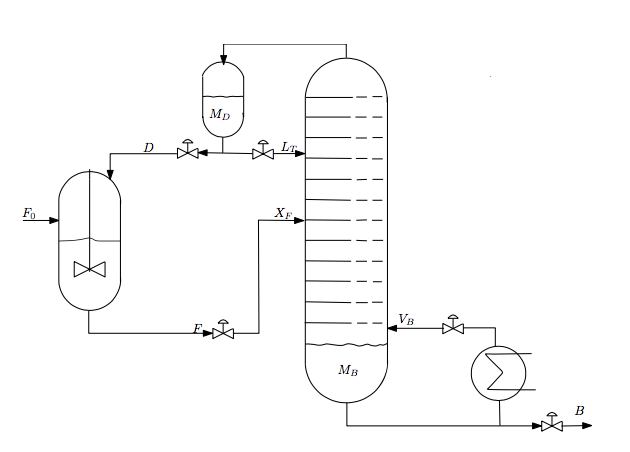
\includegraphics{process}
		\caption{Diagram of a continuously-stirred tank reactor (CSTR) and distillation column.}
		\label{fig:process}
	\end{figure}
The continuously-stirred tank reactor (CSTR) receives a stream of pure component $\mathcal{A}$ and a recycle stream $\mathcal{R}$ from the distillation column.
A first-order reaction ($\ce{\mathcal{A} -> \mathcal{B}}$) takes place in the CSTR and $\mathcal{B}$ is the desired product. 
The product is then feed with a flow rate $F$ to the distillation column where the unreacted raw material is then separated from the product and recycled to the reactor.
The desired product $\mathcal{B}$ is the bottom product and must have a certain purity.
Table \ref{tab:rxn_kin} summarizes the reaction kinetic parameters for the reactor.
\begin{table}[H]
	\centering
	\caption{Reaction kinetic parameters}
	\begin{tabular}{c c c}
		\toprule[0.3mm]\\
		\textbf{Reaction} & \textbf{Reaction Rate Constant (\si{\per\minute})} & \textbf{Activation Energy (\si{\joule\per\mole})}\\
		\midrule[0.2mm]
		$\ce{\mathcal{A} -> \mathcal{B}}$ & $1\times10^8$ & $6\times10^4$\\
		\bottomrule[0.3mm]
	\end{tabular}
	\label{tab:rxn_kin}
\end{table}
\par
The distillation column model is taken from \cite{model}.
The parameters used for the distillation column are summarized in Table \ref{tab:column}.
\begin{table}[H]
	\centering
	\caption{Distillation column parameters}
	\begin{tabular}{c c}
		\toprule[0.3mm]\\
		\textbf{Parameter} & \textbf{Value}\\
		\midrule[0.2mm]\\
		$\alpha_{AB}$ & 1.5\\
		number of stages & 41\\
		feed stage location & 21\\
		\bottomrule[0.3mm]\\
	\end{tabular}
	\label{tab:column}
\end{table}
The distillation column is comprised of 40 theoretical stages (39 trays and a reboiler) plus a total condenser.
The feed is an equimolar liquid mixture of components $\mathcal{A}$ and $\mathcal{B}$ with a relative volatility of 1.5.
The pressure $P$ is assumed constant due to perfect control of $P$ using $V_T$ as an input.
The reflux and boilup rates are such that we nominally have 99\% purity for reach product ($y_D$ and $x_B$).
The nominal holdup is $M_i^*/F=0.5$ \si{\minute} for all stages, including the reboiler and condenser.
A simple linear relationship $L_i(t)=L_i^*+(M_i(t)-M_i^*)/\tau_L$, where $\tau_L=0.063$ \si{\minute} is used to model the liquid flow dynamics on all trays.
The model uses the following assumptions: binary separation, constant relative volatility, no vapor holdup, one feed and two products, constant molar flows, and a total condenser.
Actuator and measurement dynamics are not included.
\par
The whole model (CSTR and distillation column) has a total of 84 state variables: 82 from the distillation column (mole fractions and liquid holdups from each stage) and two from the CSTR (concentration and holdup).
%%%%%%%%%%%%%%%%%%%%%%%%%%%%%%%%%%%%%%%%%%%%%%%%%%%%%%%%%%%%%%%%%%%%%
%%%%%%%%%%%%%%%%%%%%%%%%%%%%%%%%%%%%%%%%%%%%%%%%%%%%%%%%%%%%%%%%%%%%%
\subsection{Model Equations}
The basic equations used to model the CSTR and distillation column are outlined below.
The notation is outlined in Table \ref{tab:notation}.
\begin{enumerate}[label = \roman*)]
	\item Total balance on stage $i$:
		\begin{equation}
			\frac{dM_i}{dt}=L_{i+1}-L_i+V_{i+1}-V_i
		\end{equation}
	\item Material balance for light component on each stage $i$:
		\begin{equation}
			\frac{d(M_ix_i)}{dt}=L_{i+1}x_{i+1}+V_{i-1}y_{i-1}-L_ix_i-V_iy_i
		\end{equation}
		which also gives the following expression for the derivative of the liquid mole fraction:
		\begin{equation}
			\frac{dx_i}{dt}=\frac{\frac{d(M_ix_i)}{dt}-x_i\frac{dM_i}{dt}}{M_i}
		\end{equation}
	\item Algebraic equations(apply to all stages except condenser, feed and reboiler):
		\begin{itemize}
			\item Vapor-liquid equilibrium
				\begin{equation}
					y_i =\frac{ \alpha x_i}{1+(\alpha-1)x_i}
				\end{equation}
			\item From assumption of constant molar flows and no vapor dynamics (except if feed is partially vaporized):
				\begin{equation}
					V_i=V_{i-1}
				\end{equation}
			\item Linearized liquid flow:
				\begin{equation}
					L_i= L0_i+\frac{(M_i-M0)}{\tau_l}+(V-V_0)_{i-1}
				\end{equation}
				where $L0_i$ \si{\kilo\mole\per\minute} and $M0_i$ \si{\kilo\mole} are the nominal values for the liquid flow and holdup on stage $i$.
		\end{itemize}
	\item Feed stage ($i = NF$):
		\begin{align}
			\frac{dM_i}{dt}&=L_{i+1} -L_i+V_{i-1}-V_i+F\\
			\frac{d(M_ix_i)}{dt}&= L_{i+1}x_{i+1}+V_{i-1}y_{i-1}-L_ix_i-V-iy_i+Fz_F
		\end{align}
	\item Total condenser ($i = NT$):
		\begin{align}
			\frac{dM_i}{dt}&=V_{i-1}-L_i-D\\
			\frac{d(M_ix_i)}{dt}&=V_{i-1}y_{i-1}-L_ix_i-Dx_i
		\end{align}
	\item Reboiler ($i=1$):
		\begin{align}
			M_i&=M_B\\
			V_i&=V_B=V\\
			\frac{dM_i}{dt}&=L_{i+1}-V_i-B\\
			\frac{d(M_ix_i)}{dt}&=L_{i+1}x_{i+1}-V_iy_i-Bx_i
		\end{align}
\end{enumerate}
%%%%%%%%%%%%%%%%%%%%%%%%%%%%%%%%%%%%%%%%%%%%%%%%%%%%%%%%%%%%%%%%%%%%%
%%%%%%%%%%%%%%%%%%%%%%%%%%%%%%%%%%%%%%%%%%%%%%%%%%%%%%%%%%%%%%%%%%%%%
\subsection{Column data}
As mentioned above, the column has 41 stages including the reboiler and total condenser with the feed stage located at stage 21.
The nominal steady state conditions for this column are summarized in Table \ref{tab:column_data}.
\begin{table}[H]
	\centering
	\caption{Column data}
	\begin{tabular}{c c}
		\toprule[0.5mm]\\
		\textbf{Parameter} & \textbf{Value}\\
		\midrule[0.5mm]\\
		Feed rate $F$ & 1 [\si{\kilo\mole\per\minute}]\\
		Feed composition $z_F$ & 0.5 [mole fraction unit]\\
		Feed liquid fraction $q_F$ & 1 [saturated liquid]\\
		Reflux flow $L_T$ & 2.706 [\si{\kilo\mole\per\minute}]\\
		Boilup $V$ & 3.206 [\si{\kilo\mole\per\minute}]\\
		Liquid holdup $M0$ & 0.5 [\si{\kilo\mole}]\\
		Time constant for liquid dynamics $\tau_l$ & 0.063 [\si{\minute}]\\
		$\lambda$ & 0 \\
		Distillate $D$ & 0.5 [\si{\kilo\mole\per\minute}]\\
		Distillate composition $y_D=x_{NT}$ & 0.99 [mole fraction units]\\
		Bottoms $B$ & 0.5 [\si{\kilo\mole\per\minute}]\\
		Bottoms composition $x_B=x_1$ & 0.01 [mole fraction units]\\
		\bottomrule[0.2mm]
	\end{tabular}
	\label{tab:column_data}
\end{table}
This steady state data can easily be recalculated to simulate different columns (number of stages, feed composition, flows, relative volatility, holdups) by using \texttt{col\_model.py} and \texttt{col\_LV.py}. 
%%%%%%%%%%%%%%%%%%%%%%%%%%%%%%%%%%%%%%%%%%%%%%%%%%%%%%%%%%%%%%%%%%%%%
%%%%%%%%%%%%%%%%%%%%%%%%%%%%%%%%%%%%%%%%%%%%%%%%%%%%%%%%%%%%%%%%%%%%%
\subsection{Detailed LV-model}
This model is obtained from model reduction of the detailed 82 state model and only has 5 states.
It includes liquid flow dynamics, composition dynamics, and disturbances.
In this simplified case the inputs are the reflux ($L$) and boilup ($V$) and the controlled outputs are the top and bottom product compositions ($y_D$ and $x_B$).
\par
This simplified model is used to find initial steady state conditions for the distillation column to initialize the remainder of the simulation.
%%%%%%%%%%%%%%%%%%%%%%%%%%%%%%%%%%%%%%%%%%%%%%%%%%%%%%%%%%%%%%%%%%%%%
\section{Objective Function and Constraints}
The economic objective function to be optimized under operation is given by:
	\begin{equation}
		J=p_FF_0+p_VV_B-p_BB
	\end{equation}
where $p_F$ is the feed cost, $p_V$ is the steam cost and $p_B$ is the product price.
The following prices are used in this case study: $p_F=1\, \si{\$\per\kilo\mole}, p_V=0.02\, \si{\$\per\kilo\mole},\text{ and } p_B=2\, \si{\$\per\kilo\mole}$.
The constraints are the concentration of the bottom product ($x_B\leq 0.1$), the liquid holdup at the bottom and the top of the distillation column and in the CSTR ($0.3\leq M_{(B,D,CSTR)}\leq 0.7\,\si{\kilo\mole}$).
The control inputs are the reflux flow ($L_T$), boil-up flow ($V_B$), feed rate to the distillation column ($F$), distillate flow rate ($D$) and bottom product flow rate ($B$).
These control inputs have the following bounds:
\begin{equation}
	\begin{bmatrix} 0.1\\0.1\\0.1\\0.1\\0.1\end{bmatrix}\leq
	\begin{bmatrix} L_T \\ V_B\\F\\D\\B\end{bmatrix}\leq
	\begin{bmatrix} 10\\4.008\\10\\1.0\\1.0\end{bmatrix}
\end{equation}
\par
To solve this problem we must first run a steady-state optimization; we select a feed rate $F_0=0.3\, \si{\kilo\mole\per\minute}$.
This gives optimal values for control inputs and state variables at this feed rate.
The optimal steady state input values are found to be $\boldsymbol{u}_{ss}=\begin{bmatrix}1.18 & 1.92 & 1.03 & 0.74 & 0.29\end{bmatrix}^T$.
\par
The optimal state and control inputs are then used to construct a regularization term that is added to the objective function.
Regularization terms are often used in optimization problems  helps to introduce more information to the function to help solve an ill-posed problem or to prevent overfitting.
The regularization term also helps to regulate the different goals of the objective function.
The new objective function for the regularized stage is written as:
\begin{equation}
	J_m = p_FF_0 + p_VV_B-p_BB-p_DD+(\boldsymbol{z}-\boldsymbol{x}_s)^T\boldsymbol{Q}_1(\boldsymbol{z}-\boldsymbol{x}_s)+(\boldsymbol{v}-\boldsymbol{u}_s)^T\boldsymbol{Q}_2(\boldsymbol{v}-\boldsymbol{u}_s)
\end{equation}
The weights ($\boldsymbol{Q}_1$ and $\boldsymbol{Q}_2$) are selected to make the rotated stage cost of the steady state problem strongly convex. 
To find a valid diagonal regularization matrix $Q$ we utilize the Gershgorin property for a matrix which states for a matrix $\boldsymbol{A}=(a_{ij})$:
	\begin{equation}
		a_{ii}-\sum_{i\neq j}|a_{ij}|\leq \mu_i\leq a_{ii}+\sum_{i\neq j} |a_{ij}|
	\end{equation}
where $\mu_i$ are the eigenvalues of $\boldsymbol{A}$\cite{fast}.
This property can be utilized to systematically find the regularization terms such that the rotated stage cost will be strongly convex and thus
a stable economic NMPC controller can be obtained using this method.
For further details on this method see \cite{fast}.
\par
The distillation column is initialized using the steady states values for a feed rate of $F_0 = 0.29$ \si{\kilo\mole\per\minute} meaning that the controller is essentially controlling for a throughput change from $F_0 = 0.29$ \si{\kilo\mole\per\minute} to $F_0 = 0.30$ \si{\kilo\mole\per\minute}.
The simulation is run for 150 MPC iterations with a sample time of 1 minute.
The prediction horizon of the NMPC controller is set to 30 minute.
This results in an NLP with 10,314 optimization variables (\cite{economic}).
To solve the NLP, CasADi with IPOPT is used; for the QPs, we use CasADi with qpoases (\cite{Andersson2013b}).

